\section{Zweiter Entwurf}

\subsection{Entwurfsziele}
Im zweiten Entwurf sollen die Ideen aus dem vorherigen Abschnitt möglichst effizient umgesetzt werden.
Das heißt der Beschleuniger wird in zwei Atome aufgeteilt, um die Datenmenge in einem Atom zu reduzieren
und statt der Standard-Rundenfunktion wird die erweiterte Rundenfunktion in den zwei Teilschritten Gamma und Rho implementiert.
Damit die Komponenten miteinander arbeiten können und die Atome Daten miteinander austauschen können, braucht es zusätzlich noch
einen Zustandsautomaten, der das Verhalten der Komponenten kontrolliert.
Die Atome sollen so klein sein wie möglich und dürfen dabei ruhig ein wenig die Ausführungszeit erhöhen.
Ziel des Entwurfs ist es die bisherigen Überlegungen zu testen und sicher zu stellen, dass sie die gewünschte Auswirkung zeigen.
\begin{figure}
	\center
	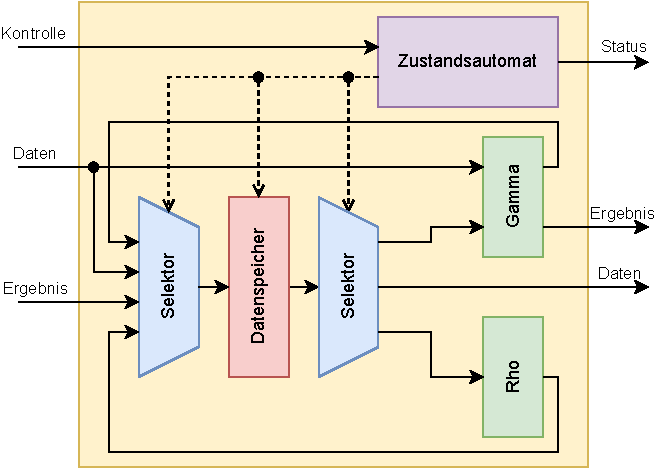
\includegraphics{images/Iteration_2.pdf}
	\caption{Atomaufbau des zweiten Entwurfs}
	\label{fig:aufbau_iteration_2}
\end{figure}
\subsection{Aufbau}
Der Beschleuniger ist in zwei Atome aufgeteilt (Abb. \ref{fig:aufbau_iteration_2}), die jeweils einen Teil des Datenblocks speichern. Beide Atome sind gleich aufgebaut, erst über ein Bit im Kontrollvektor,
den sogenannten \textbf{Atom-Index}, wird festgelegt als welcher Teil des Beschleunigers ein Atom arbeitet. Die Daten sind dabei spaltenorthogonal aufgeteilt, sodass die Lanes 0 bis 12 in Atom 0,
und die Lanes 12 bis 24 in Atom 1 gespeichert werden (Abb. \ref{fig:datenaufteilung}). Die Lane 12 wird dabei absichtlich doppelt gespeichert,
damit beide Atome 13 Lanes speichern, wodurch der gleiche Aufgebaut ermöglicht wird. Jedes Atom speichert somit 13 Lanes aus jeweils 64 Bits, also insgesamt 832 Bits.
Diese Daten werden in einem Block aus FFs gehalten. Über einen Selektor werden aus diesem Datenspeicher die Daten für die Berechnungsblöcke Rho und Gamma sowie für die Kommunikation ausgewählt.
Die Ergebnisse der Berechnungsblöcke sowie die empfangenen Daten werden über einen weiteren Selektor zusammengefügt und wieder im Datenspeicher gespeichert.
Welche Daten von den Selektoren ausgewählt werden und welche im Speicher übernommen werden, bestimmt ein Zustandsautomat. Dieser wird über einen Kontrollvektor von außen gesteuert
und koordiniert die einzelnen Berechnungsschritte und sorgt dafür, dass das Kommunikationsprotokoll befolgt wird.

\subsection{Ablauf einer Berechnung}
\subsubsection{Dateneingabe}
Über den Datenbus werden die Atome mit den Eingabedaten versorgt. Die Eingabe wird entsprechend mit den bereits gespeicherten über ein XOR kombiniert.
Auf diese Weise können der Schwammkonstruktion entsprechend neue Datenblöcke direkt in den Atomen aufgenommen werden ohne,
dass das Ergebis der vorherigen Berechnung erst gelesen werden muss.
\subsubsection{Rho}
Für die Berechnung von Rho werden alle Lanes in einem Atom gleichzeitig in einem Takt wie in einem Schieberegister entsprechend rotiert.
\subsubsection{Gamma}
Die Berechnung von Gamma wird in mehrere Teilschritte aufgeteilt. Atom 0 ist dabei für die Berechnung der Slices 0 bis 31 zuständig und Atom 1
führt die Berechnung für die Slices 32 bis 63 durch. Damit ein neuer Slice berechnet werden kann, muss der vollständige Slice im Atom vorliegen.
Da jeweils 13 Bit schon im eigenen Datenspeicher vorhanden sind, müssen noch 12 Bits aus dem Speicher des anderen Atoms übertragen werden.
Nach der Berechnung muss das Ergebnis in beiden Atomen übernommen werden. Dafür müssen wieder 13 Bits pro Slice übertragen werden.
Um das Kommunikationsprotokoll so einfach wie möglich zu halten und die Ausführungszeit zu minimieren, wird die Berechnung ge-pipelined.
Der 64 Bit breite Voll-Duplex-Kanal zwischen den Atomen wird aufgeteilt in einen 32 Bit breiten Datenkanal und einen 32 Bit breiten Ergebniskanal.
Der genaue Berechnungsverlauf ist noch einmal im Schaubild [Bild Nr] erklärt.
[Schaubild]
\begin{enumerate}
\item Die Daten für Atom 1 werden aus dem Datenspeicher gelesen und an den Datenkanal angelegt.
\item Die Daten für Atom 1 befinden sich im Register des Datenkanals
\item Die Daten für Atom 1 sind am Atom eingetroffen. Gleichzeitig treffen auch die von Atom 1 gesendeten Daten an Atom 0 ein.
Die erhaltenen Daten werden mit den Daten aus dem Speicher von Atom 0 zu vollständigen Slices kombiniert und der Berechnungseinheit bereitgestellt.
\item Die Berechnungseinheit berechnet das Ergebnis und gibt es zurück.
\item Das Ergebnis wird im Datenspeicher übernommen und die Hälfte, die in Atom 1 gespeichert werden soll, wird am Ergebniskanal angelegt.
\item Das Erbebnis im Ergebnisbus befinden sich im Register des Ergebniskanals
\item Das Ergebnis trifft in Atom 1 ein. Gleichzeitig trifft auch das Ergebnis von Atom 1 in Atom 0 ein.
Das erhaltene Ergebnis wird im Datenspeicher übernommen.
\end{enumerate}
Die maximale Anzahl an Slices, die gleichzeitig in einem Atom berechnet werden kann, ergibt sich in diesem Fall aus der stark beschränkten Bandbreite
des Kommunikationskanals. In dem 32 Bit breiten Kanal können maximal zwei 12 Bit bzw 13 Bit Einträge in einem Takt übertragen werden.
Um den gesammten Blockteil zu berechnen, muss die oben aufgeführte Berechnungsabfolge also 16 Mal mit jeweils 2 Slices durchgeführt werden.
Da die Berechnung der 7 Schritte in einer Pipeline durchgeführt wird, beträgt die Berechnungsdauer nicht 16 * 7 = 112 Schritte,
sondern nur 7 + (16 - 1) = 22 Schritte.

\subsection{Bewertung}
Die Ausführungszeit für eine Iteration der modifizierten Rundenfunktion ist wie erwartet etwa um einen Faktor 30 langsamer als die Implementierung der ersten Iteration.
Dies ist wie bereits erklärt hauptsächlich der Aufteilung der Gamma-Funktion in 16 Teilschritte geschuldet, sowie der damit einhergehenden Verzögerung.
Anders jedoch als erwartet, ist die Größe der Atome durch das Aufteilen der Berechnung und des Datenspeichers nicht wie gewünscht gesunken.
Tatsächlich ist der Entwurf mit seinen etwa 4600 LUTs nochmal um gut 37\% größer. Dafür gibt es zwei wesentliche Gründe: den Zustandsautomaten sowie die Speicherkomplexität,
die in der Überlegung für das Design nicht bedacht wurden.
\subsubsection{Zustandsautomat}
Der Zustandsautomat besteht aus einem Iterator, der in jedem Takt hochgezählt wird und anhand dessen die Steuersignale für die anderen Komponenten genertiert werden.
Entgegen der ursprünglichen Annahme, dass seine Größe aufgrund der Einfachheit der Aufgabe vernachlässigbar ist, nimmt er in diesem Design etwa 300 LUTs ein.
Auch wenn sich die konkrete Implementierung noch optimieren lässt, so ist klar geworden, dass die weitere Erhöhung der Berechnungskomplexität mit Bedacht durchgeführt werden muss,
da der Zustandsautomat dadurch nur noch größer wird.
\subsubsection{Schreib- und Lesemuster}
Im ersten Entwurf wird der Wert jedes Bits im Register entweder von der Eingabe oder von der Ausgabe der Rundenfunktion bestimmt.
Im zweiten Entwurf hingegen hängt dieser Wert ab von der Eingabe, des Ergebnisses der Rho-Rotation sowie einem Bit im Ergebnis-Kanal.
Welches Bit aus dem Ergebniskanal für ein Bit im Datenspeicher bestimmt ist, legt der Zustandsautomat und auch der Atom-Index fest.
Diese Auswahlschaltung sowie die Entscheidung, wann genau das Bit im Register überschrieben werden muss (im ersten Entwurf wurden einfach alle Bits in jedem Takt überschrieben, wenn das Kontrollsignal aktiv war),
benötigen schon mehr Platz als die Reduktion der Datenmenge einspart.
Analog ist auch das Lesen der Daten komplizierter geworden. Die Gamma-Funktion sowie der Datenkanal müssen anhand des Zustandsautomaten und des Atom-Indexes aus allen Bits nur ein par auswählen.
\subsubsection{Gamma-Funktion}
Die Gamma-Funktion übernimmt bis auf Rho alle Subfunktionen der Standard-Rundenfunktion. Da die Berechnung auf zwei Atome aufgeteilt ist und auch nicht alle Slices in einem Atom gleichzeitig berechnet werden,
ist die Komplexität der Gamma-Funktion sehr stark geschrumpft, sodass das aktuelle Design nur etwa 70 LUTs benötigt. Eine weitere Optimierung der Gamma-Funktion ist daher auch in weiteren Iterationen nicht mehr nötig.

\subsection{Optimierungsansätze}
Die starke Steigerung der Speicherkomplexität ist das Hauptproblem des Entwurfs und weitere Verbesserungen müssen hier ansetzen, um den Beschleuniger aus die erforderliche Größe reduzieren zu können.
Um die Speicherverwaltung vollständig aus dem Design zu entfernen, hatten wir die Nutzung der BRAM-Blöcke in den Überlegungen des ersten Entwurfs schon einmal erwähnt und uns letztendlich dagegen entschieden,
weil das Festlegen auf einen Tile-orientierten Speicher bedeutet, dass die Rho-Funktion, die eigentlich auf Lanes arbeitet, so implementiert werden muss, dass sie mit Tiles arbeiten kann.
\subsubsection{Transformation der Rho-Funktion}


\subsubsection{BRAM als Datenspeicher}
